\Chapter{Megvalósítás}

A megvalósítás a már előző fejezetben tervezett struktúrát követte. Ebben a fejezetben néhány modul érdekesebb részeit fogom bemutatni, amelyek implementáció szempontjából nem biztos, hogy triviálisak.

\Section{linux modul érdekességei}

A legelsők közt készült el a \textit{linux} modul megvalósítása, mivel több modul is függött a funkcionalitásától. Néhány érdekesebb részt szeretnék bemutatni, mint például az \texttt{exists}, \texttt{isdir} implementációját:

\begin{lua}
function module.exists(file)
    local ok, err, code = os.rename(file, file)
    if not ok then
		return code == 13 or code == 17
    end
    return ok, err
end
function module.isDir(path)
    return module.exists(path.."/")
end
\end{lua}

Ez a kód úgy nézi meg a fájlok létezését, hogy megpróbálja a fájlokat átnevezni saját magukra. Ekkor kétféle error lehetséges: \textbf{Permission Denied} (code 13) vagy \textbf{File exists} (code 17). Jegyzékek létezését pedig úgy ellenőrzi, hogy hozzárakja a path végéhez a \textit{/} jelet, mivel így biztos, hogy jegyzékre mutat a path.

Érdekes lehet még az \texttt{\detokenize{execCommand}} és a \texttt{\detokenize{execCommandWithProcRetCode}} funkció implementációja is. Ezek a funkciók a program gerincét képezik, a legtöbb modul használja őket.

\begin{lua}
function module.execCommand(cmd)
    local handle = io.popen(cmd);
    local result = handle:read("*a");
    handle:close();
    return result;
end
\end{lua}

Az \texttt{\detokenize{execCommand}} egyszerű implementációjú, amely az \textit{io} standard library popen funkcióját használja meg egy processz megnyitására. Ez egy handlet ad. A read megvárja míg lefut a processz, majd az \textit{\detokenize{*a}} paraméter segítségével mindent kiolvas a pipeból. A végén lezáródik a handle. Windows rendszeren is tökéletesen működik.

A következő funkció az \texttt{\detokenize{execCommandWithProcRetCode}}. Itt a forráskódból kivettem az üres sorokat a kompaktabb kód érdekében. Működése nagyban hasonlít az \texttt{\detokenize{execCommand}}-hoz, azzal a kivétellel, hogy ez az implementáció felhasznál bizonyos Bash-script elemeket. Például az \textit{export} funkciót az environment variablek beállítására, vagy a \textit{\detokenize{$?}} változót a process return kód lekérésére. Támogatja az stderr átirányítását is stdout-ba (ez a \texttt{\detokenize{2>&1}} paraméter) cross-platform módon, a többi Bash alapú megoldás kivételével. A return code-t az utolsó sorba iratja ki, ezt olvassa be magától, és vágja ki az alap program outputjából.
\begin{lua}
function module.execCommandWithProcRetCode(cmd, linesReturned, envVariables, redirectStdErrToStdIn)
    local exportCmd = "";
    if envVariables then
        for k, v in pairs(envVariables) do
            exportCmd = exportCmd.." export "..tostring(k).."="..tostring(v).."; ";
        end
    end
    local handle = io.popen(exportCmd..cmd..tostring(redirectStdErrToStdIn and " 2>&1" or "").."; echo $?");
    handle:flush();
    local overallReturn = "";
    local lastLine = "";
    local newLineChar = "\n";
    local lineNum = 0;
    for line in handle:lines() do
        overallReturn = overallReturn .. line .. newLineChar;
        lastLine = line;
        lineNum = lineNum + 1;
    end
    handle:close();
    local retCode = tonumber(lastLine);
    if lineNum == 1 then
        overallReturn = "";
    else
        overallReturn = string.sub(overallReturn, 1, #overallReturn - #lastLine - #newLineChar * 2); --skip return code line
    end
    if linesReturned then
        return overallReturn, retCode;
    end
    return retCode;
end
\end{lua}

\pagebreak
\SSubSection{Processzek visszatérési értékeinek felhasználása}{Processzek visszatérési értékei}
Valamennyi funkció a programban kihasználja azt, hogy a processzek egy meghatározott visszatérési értéket (pontosabban \textit{exit code}-t) adnak vissza lefutásuk után. Ezeknek jelentőségük van, mivel bizonyos műveleteknél más értékeket adhatnak vissza attól függően, hogy milyen funkcionalitást használunk épp. Találhatunk olyan listát az Interneten, amelyek ezeket a kódokat általánosságban írják le, hogy milyen hibához kapcsolódhatnak. 
Általában a processzek visszatérési értékeinek jelentése valamennyire hasonlít a legtöbb táblázatban hozzákapcsolt leíráshoz. \cite{linux_exitcodes}

A legfontosabb, hogy általában a legtöbb processz \textit{0}-s értékkel fog visszatérni, ha sikeresen lezajlott a a processz futása, hiba nélkül. Ezt több programrész is felhasználja, például:

\begin{lua}
function module.checkIfUserExists(userName)
    local retCodeForId = module.execCommandWithProcRetCode("id "..userName);
    return retCodeForId == 0;
end
\end{lua}

Ebben az esetben a \texttt{\detokenize{checkIfUserExists}} funkció az alapján tudja egy felhasználó létezését, hogy \textit{0}-s exit code-val tért-e vissza az \textit{id} processz.

Vagy másik példaként az \textit{mkdir} parancs \textit{0}-s (néhány táblázat szerint: \textbf{Success}) visszatérési értékkel tér vissza akkor, ha sikerült létrehozni egy új jegyzéket, vagy \textit{1}-es (néhány táblázat szerint: \textbf{Operation not permitted}) visszatérési értékkel tér vissza akkor, ha már létezik az a jegyzék, amit létre szeretnénk hozni. A programkód is ez alapján dönti el, hogy sikeres-e a jegyzék létrehozása:
\begin{lua}
function module.mkDir(path)
    local retCodeForMkdir = module.execCommandWithProcRetCode("mkdir "..path);
    return retCodeForMkdir == 0 or retCodeForMkdir == 1; --new dir successfully created/already exists
end
\end{lua}

Ez szintén hasonlóan működhet olyan programoknál is, amelyek nem rendszerprogramok, hanem valaki más készítette őket. Például a \textit{certbot} is különböző processz visszatérési értékkel térhet vissza az adott művelet sikerességétől függően:
\begin{lua}
function module.trySSLCertificateCreation(method, domain, webserverType)
    ...
    local retLines, retCode = linux.execCommandWithProcRetCode("certbot certonly -n "..tostring(dryRunStr).." --agree-tos --no-eff-email --email \"\" --webroot --webroot-path "..tostring(websiteData.rootPath).." -d "..tostring(domain), true, nil, true);
    ...
    local hasCertificate = retCode == 0;
    ...
end
\end{lua}

\pagebreak
\Section{Háttérben futó processz eredményeire való várás}

A program tervezése, implementálása során belefutottam egy nehézségbe, amely a Lua alapvető kialakításából fakad: a Lua alapvetően egy szálon fut, és nem eseményalapú felépítésű. Létezik \textit{coroutine} beépített library, azonban az \textit{könnyű szál} alapú implementáció. Egyszerre csak egy coroutine futhat, és maga a coroutine kezdeményezheti azt, hogy épp felfüggesztve, suspendelve legyen (tehát visszaadja az irányítást az őt futtató kódnak, vagy más coroutinenak). Emiatt a coroutine sem volt megoldás erre a nehézségre.

A \textit{certbot} modul tervezése, implementálása közben jött elő ez a nehézség. A \textit{HTTP-01} challenget könnyen lehetett implementálni úgy, hogy megvártuk az újonnan létrehozott processz futási eredményeit, mivel az támogatta a nem-interaktív módot. Azonban a \textit{DNS-01} challenget nem lehet ilyen könnyen implementálni.

A probléma ott kezdődött, hogy a \textit{certbot} maga alapvetőleg sajnos nem támogatja azt, hogy nem-interaktív módon fut ezen challenge esetében. Megoldást azonban az jelentett, hogy \textit{\detokenize{--manual}} módban használjuk, és megadjuk neki a preferált challenget (vagyis a dns-t), továbbá \textit{manual-auth-hook} scriptet használunk. 

Ezzel a probléma felét már sikerült orvosolnunk, azonban előjött egy újabb probléma: az io.popen esetén a program megvárja a processz futásának végét. Ez azonban nekünk nem megfelelő, mivel akkor teljesen befagy a program, a DNS challenge futtatásakor pedig a felhasználónak meg kell jelenítenünk bizonyos adatokat, hogy milyen DNS rekordokat hozzanak létre a saját domainjükön és milyen értékekkel. Az \textit{os} függvénykönyvtárban található \texttt{execute} funkció másképp működik, hátránya, hogy alapvetően ez is blocking funkció, továbbá nem is tudjuk pontosan, hogy sikerült-e a program elindítása, csak akkor, ha van visszatérési értéke és megvizsgáljuk azt.
Ezután azzal folytattam a probléma megoldását, hogy Bash szkript elemeket használtam fel a program futtatásához, például a \texttt{\detokenize{&}} szimbólumot a háttérben való futáshoz, \textit{\detokenize{$?}} szimbólumot a státusz kód megkapásához, továbbá \textit{\detokenize{$!}} szimbólumot az újonnan elindított program folyamatazonosítójának megkapásához. Ezt az egészet egy nagy parancsba foglaltam. A parancs több fájlt is felhasznál:
\begin{itemize}
    \item Egy ideiglenes fájlt abból célból, hogy az újonnan létrehozott processz, továbbá a mostani processz kommunikálni tudjon egymással. Amint lefutott a certbot, ide kerül mentésre a visszatérési értéke,
    \item Egy másik ideiglenes fájlt abból a célból, hogy az újonnan létrehozott processz stdoutját és stderr pipeját abba irányítjuk, így a mostani processz tudja a kimenetet vizsgálni,
    \item Egy certbot\_pid.txt fájlt, amelyből tudjuk, hogy sikeresen lefutott-e a programunk. Azt a célt is szolgálja, hogy ha esetleg megszakadt a program futása valami miatt, akkor a következő lefutáskor a kill parancs segítségével megszüntessük a már nem használt processzt.
\end{itemize}

A kommunikáció maga a két processz között úgy történik, hogy elindul az auth Lua szkript a certbotban, amely megkapja környezeti változókon keresztül a certbottól az adatokat. Ezeket az adatokat a legelsőnek létrehozott ideiglenes fájlba írja bele, majd ezután 1 másodpercenként folyamatosan kiolvassa a tartalmát. Ez azért fontos, mert addig is blokkolja a certbot processzt, így nem halad tovább.\\Amint a felhasználó késznek nyilvánította a DNS rekordot, akkor ebbe az ideiglenes fájlba beleírodik a "ready" szó, majd ezután fut le csak a certbot DNS challengeje (megszakad a while true ciklus).

A Lua kódból néhány részletet kiemelve így néz ki az implementáció:
\begin{lua}
function module.trySSLCertificateCreation(method, domain, webserverType)
    ...
    local tempFileName = os.tmpname();
    local tempFileNameForStdOut = os.tmpname();

    local certbotPIDStuff = general.readAllFileContents("certbot_pid.txt");

    if certbotPIDStuff then
        os.execute("kill -9 "..tostring(certbotPIDStuff));
    end

    linux.deleteFile("certbot_pid.txt");

    local formattedCmd = "(certbot certonly -n "..tostring(dryRunStr).." --agree-tos --no-eff-email --email \"\" --manual --preferred-challenges dns --manual-auth-hook \"sh ./authenticator.sh \""..tostring(tempFileName).."\"\" -d "..tostring(domain).." > \""..tostring(tempFileNameForStdOut).."\" 2>&1; echo $? > \""..tostring(tempFileName).."\") & echo $! > certbot_pid.txt";
    os.execute(formattedCmd);

    if not linux.exists("certbot_pid.txt") then
        return module.EXEC_FAILED;
    end
    ...
    --fajlolvasas, cleanup
    ...
end
\end{lua}

Authentikátor szkript részlet:
\begin{lua}
while true do
    local fileHandle = io.open(fileName, "r");
    if fileHandle then
        local readStr = fileHandle:read("*a");
        fileHandle:close();
        if readStr:find("ready", 0, true) == 1 then
            break;
        end
    end
    sleep(1);
end
\end{lua}
\pagebreak
\Section{Konfigurációs fájlok módosításának implementációja}

A konfigurációs fájlok módosításához többféle modul is implementálva lett, ezeket a Tervezés című fejezetben meg is említettem: \textit{\detokenize{apache_config_handler}},\\\textit{\detokenize{nginx_config_handler}} és \textit{\detokenize{OpenVPN_config_handler}}. Ezek közül a modulok közül a legtöbb OO alapelveket igyekezett követni, az OpenVPN config handler kivételével.

A konfiguráció író és olvasó modulokat hasonlóképp ugyanarra a kódbázisra építettem fel, ez az Apache szerver \textit{envvars} fájl kezelőjének kivételével sikerült is. Mindegyik beolvasás kimenete általában két nagyobb táblából épül fel: \textit{\detokenize{parsedLines}} és \textit{\detokenize{paramToLine}}.
A \textit{parsedLines} maga az állapot tábla, abba van benne minden egyes beolvasott és értelmezett sor, benne paraméterek, kommentek vannak. A \textit{paramToLine} tábla általában csak gyorsítótár, azt mutatja meg, hogy bizonyos paraméterek hol vannak elhelyezkedve a parsedLines táblán belül, így nem kell átfésülni az egész parsedLines táblát egy adott paraméter keresésekor.

\SubSection{OpenVPN config parser-writer implementáció felépítése, használata}
A \textit{parsedLines} felépítése OpenVPN esetén egyszerű tömb, minden tömb elem egy tábla, amelyben a következő paraméterek szerepelhetnek:

\begin{itemize}
    \item \textbf{params}: Ez tartalmazza az adott paramétereket, opciókat egy adott sorban. A táblában található \textit{val} érték maga a paraméter értéke (vagy akár a konfigurációs beállítás neve), a \textit{state} pedig kifejezi az idézőjeltípust, ha használnak (ami lehet \textit{reading\_quoted\_param} \detokenize{"} esetén, vagy \textit{reading\_squoted\_param} \detokenize{'} esetén),
    \item \textbf{comment}: Ez tartalmazza az adott sorban található kommentet. Ha a \textit{params} tábla nem létezik, akkor maga az egész sor egy komment sor, ha létezik, akkor pedig a paraméterek után van a komment elhelyezve. Üres sor, ha ez sem létezik.
\end{itemize}

Kódrészlet OpenVPN szerver konfiguráció összeállítására a programból:

\begin{lua}
function module.checkServerConfig(homeDir, openVPNConfigDir)
...
    local configFileContent, paramsToLines = config_handler.parseOpenVPNConfig(sampleConfigFileContent);
    if paramsToLines["user"] then
        local paramTbl = configFileContent[paramsToLines["user"]];
        paramTbl["params"][2].val = module["openvpn_user"];
    end
...
    configFileHandle:write(config_handler.writeOpenVPNConfig(configFileContent));
    configFileHandle:flush();
    configFileHandle:close();
...
end
\end{lua}
\pagebreak

Az előző oldalon látható kódrészlet egy teljesen új konfigurációs fájlt generál az OpenVPN szerver számára. Ezt úgy teszi meg, hogy egy előre megadott alap konfigurációt beolvas, majd azon módosítja a paramétereket (például az user beállítást), utána pedig rendes konfigurációs szöveggé alakítja a módosított konfigurációt az állapot táblából. Az átírt argumentum \myaref{fig:openvpn_config_edit_example} ábrán látható.

\begin{figure}[h]
\centering
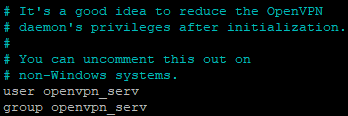
\includegraphics[scale=1.0]{images/openvpn_config_edit_example.png}
\caption{Az átírt \detokenize{user} argumentum. A példa konfigurációban nobody van használva}
\label{fig:openvpn_config_edit_example}
\end{figure}

\SubSection{Apache, nginx config parser-writer implementáció}

Az \textit{\detokenize{apache_config_handler}}, és az \textit{\detokenize{nginx_config_handler}} modulok már OO alapelveket követnek, azonban itt is fontos a két tábla felépítése. Az OpenVPN szerverhez képest a két szerver konfigurációs fájljai bonyolultabb és kiterjedtebb szintaxisú. Bár a konfigurációs fájl értelmező és író ugyanúgy két táblával dolgozik, megfigyelhető, hogy sokkal több paramétert tartalmaz egy adott sort leíró tábla.

A \textit{parsedLines} felépítése Apache és nginx esetén szintén egyszerű array, minden array elem egy tábla (és egy sor), amelyben a következő paraméterek szerepelhetnek (akár több is egyszerre):

\begin{itemize}
    \item \textbf{spacer}: Üres sort jelent. Ha ez létezik, akkor a többi lentebb sorolt paraméter biztosan nem létezik az adott elemtáblában,
    \item \textbf{blockStart}: Egy blokk kezdetét jelenti, a blokk azonosítóját tartalmazza. Apache esetében argumentumok is tartozhatnak hozzá (tehát ilyenkor az args paraméter is feldolgozódik),
    \item \textbf{blockEnd}: Egy blokk végét jelenti, a lezárandó blokk azonosítóját tartalmazza,
    \item \textbf{paramName}: Adott sorban található beállítás nevét tartalmazza (például nginx esetében include, Apache esetében ServerName), egy táblában, amely ugyan úgy épül fel, mint az args paraméter. Természetesen mellé feldolgozódik az args paraméter is.
    \item \textbf{comment}: Ez tartalmazza az adott sorban található kommentet. Ha az \textit{args} tábla nem létezik, akkor maga az egész sor egy komment sor, ha létezik, akkor pedig a paraméterek után van a komment elhelyezve nginx esetén. Az Apache nem támogat kommenteket a sorok végén, az optionok és argumentumok után,
    \item \textbf{blockDeepness}: Megadja, hogy az adott sor mennyire van eltolva indent-ügyileg,
    \item \textbf{args}: több elem esetében is használatos paraméter (például Apache esetében blockStartnál is, paramName-nél pedig mindkettő implementációnál), amely egy tábla, és az adott művelethez tartalmaz paramétereket:
        \begin{itemize}
            \item \textbf{quoteStatus}: lehet \textit{d}, ekkor duplaidézőjelben van a paraméter; lehet \textit{s}, ekkor két sima idézőjel között van a paraméter,
            \item \textbf{multipleLine}: Apache esetében használatos, ha egy paraméter több sort is magába ölel (Apache-ban támogatott a több sor a \texttt{\detokenize{\\}} jelölés segítségével),
            \item \textbf{data}: ez maga egy szöveg, amely a paraméterhez tartozó adatokat tartalmazza.
        \end{itemize}
\end{itemize}

A két modul használata valamelyest eltér az előző OpenVPN konfigurációt kezelő modultól. Ezek már OO alapelveket követnek, továbbá valamennyivel több funkciót is implementálnak, szélesebb körben vannak használva a programban. Például van implementálva funkció arra, hogy teljesen új adatot tudjunk beszúrni bárhova, erre az OpenVPN szerver kezelő implementációja közben nem volt szükség.

A következőekben két rövid kódrészletet fogok mutatni Apache és nginx esetében is a modulok használatáról. Nginx esetében a következőképp kerül beállításra az SSL egyik beállítása:
\begin{lua}
function module.initSSLForWebsite(webUrl, certDetails)
    ...
    --Redirect unencrypted connections
    local blockName = 'if ($scheme != "https")';
    local blockStartSchemeIdx = paramsToIdx["block:"..tostring(blockName)];
    if not blockStartSchemeIdx then
    local blockDeepness = serverNameData.blockDeepness;
        configInstance:insertNewData({["comment"] = " Redirect unencrypted connections", blockDeepness = serverNameData.blockDeepness}, posStart);
        posStart = posStart + 1;
        configInstance:insertNewData({["blockStart"] = blockName, block = serverNameData.block, blockDeepness = serverNameData.blockDeepness, args = {}}, posStart);
        posStart = posStart + 1;
        blockDeepness = blockDeepness + 1;
        configInstance:insertNewData({["paramName"] = {data = 'rewrite'}, block = blockName, blockDeepness = blockDeepness, args = {{data = "^"}, {data = "https://$host$request_uri?"}, {data = "permanent"}}}, posStart);
        posStart = posStart + 1;
        blockDeepness = blockDeepness - 1;
        configInstance:insertNewData({["blockEnd"] = blockName, block = serverNameData.block, blockDeepness = serverNameData.blockDeepness, args = {}}, posStart);
        posStart = posStart + 1;
    end
    ...
end
\end{lua}
A kódrészlet megkeresi a \detokenize{'if ($scheme != "https")'} blokkot az adott weboldal nginx-konfigurációjában. Ha nem találja meg beszúr egy kommentet, majd azután beszúr egy blokk-kezdést. A blokkba beilleszti a \detokenize{'rewrite ^ https://$host$request_uri? permanent'} parancsot, majd lezárja a blokkot a parancs után. Mindezeket indentálva teszi, így a konfiguráció jól átlátható marad. A beállítás maga azt jelenti, hogy minden HTTP-n keresztüli csatlakozást átirányít HTTPS-re.

A gyakorlatban \myaref{fig:inserted_block_nginx} ábrán látható módon néz ki a beillesztett blokk, az nginx konfigurációjában.
\begin{figure}[h]
\centering
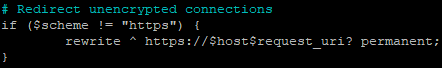
\includegraphics[scale=1.0]{images/nginx_config_edit_example.png}
\caption{A beillesztett blokk}
\label{fig:inserted_block_nginx}
\end{figure}

Apache esetében is hasonlóan működik a konfiguráció módosítása. Ott azonban teljesen külön blokkot kell csinálni az SSL konfigurációnak, teljesen új beállításokkal, továbbá a jelenlegi beállítások hozzáfűzésével, ezért az azt beállító kódrészlet hosszabb az nginx-implementációtól. Rövid kódrészlet az Apache SSL beállításából:
\begin{lua}
function module.initSSLForWebsite(webUrl, certDetails)
    ...
    blockDeepness = blockDeepness + 1;
    configInstance:insertNewData({
        blockStart = "VirtualHost",
        args = {
            {data = "*:443"}
        },
        blockDeepness = blockDeepness
    });
    ...
    configInstance:insertNewData({
        paramName = {data = "Include"},
        args = {
            {data = pathForLetsEncryptApacheConfig, quoteStatus = "d"},
        },
        blockDeepness = blockDeepness
    });
    ...
    blockDeepness = blockDeepness - 1;
    configInstance:insertNewData({
        blockEnd = "VirtualHost",
        blockDeepness = blockDeepness
    });
    ...
end
\end{lua}

\pagebreak

A példakódban a VirtualHost blokk létrehozását láthatjuk, amelybe egy Include beállítás is beszúrásra kerül. Ezután lezárásra kerül a létrehozott VirtualHost blokk. A valóságban azonban az SSL beállítása sokkal több beállítást, paramétert tartalmaz, a példaként szolgáltatott \myaref{fig:newly_inserted_apache_block} ábra csak a kiragadott példakód funkcionalitását kívánja bemutatni.
\begin{figure}[t]
\centering
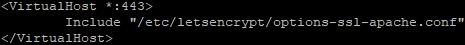
\includegraphics[scale=1.0]{images/apache_config_edit_example.png}
\caption{A kiragadott példakód által generált konfiguráció}
\label{fig:newly_inserted_apache_block}
\end{figure}

\Section{Modulok használata Lua-ban}

Az összes modul, továbbá a main.lua-ban található felhasználói interface is különböző modulokat használ fel. Ezeket a modulokat a \texttt{require} funkcióval lehet betölteni. A \texttt{require} funkció működése hasonló a \texttt{dofile} funkcióhoz, azonban két főbb különbség is van köztük. 

Az egyik az, hogy a require funkció egy megadott path-on belül keresi a betöltendő fájlt, a másik pedig, a require funkció nem engedi ugyanazon fájl duplikált betöltését. Tehát ha már egyszer betöltöttünk egy modult, akkor nem tölti be mégegyszer teljesen, hanem elcachezi egy táblában a már betöltött fájlt. Ha azonban több virtuális path-ot (például: \texttt{\detokenize{?;?.lua}} foo.lua helyett), nevet használunk ugyanazon fájlra, akkor többször is betöltődnek, mivel más lesz a fájl neve, viszont a tartalom ugyan az marad. \cite{require}

A program kódjában a main.lua-ban van megadva, hogy milyen megadott path mentén keresi meg az adott betöltendő fájlt:

\begin{lua}
package.path = package.path..";modules/?.lua";
\end{lua}

Ez a sor szimplán hozzáfűzi a package-k betöltésének pathjához a modules mappát.

Emiatt lehetséges az, hogy nem kell a .lua extensiont kiírnunk a require meghívásaink végén, továbbá, hogy tudunk modulokat betölteni például így:
\begin{lua}
local OpenVPNHandler = require("vpnHandler/OpenVPN");
local linux = require("linux");
\end{lua}

A require funkció a háttérben a megadott fájl kódját futtatja le. Így működik például a \textit{Client} class implementációja az összes modulban is, amelybe be van töltve a config handler, mivel a Client tábla globális változó. 

Minden fájl egy adott code-scope, azonban a globális változók hozzáférhetőek azokban a modulokban is, amelyek betöltötték az adott modult. Emiatt lehetséges például a lokálisan definiált funkciók, változók szeparációja. Az adott modulok a saját maguk kódjában használják őket, viszont az őt betöltő modulok már nem tudnak hozzáférni ezekhez a funkciókhoz, változókhoz.

Modulok esetében a saját implementációmban egy lokális tábla hozódik létre (tehát alapvetőleg "private" láthatóságú), azonban mégis tudjuk használni azt. Ez azért van, mert a require funkció az adott kód lefutási értékét adja vissza. Így lehet akár funkcióval is visszatérni, ami konstruktorként szolgálhat (és az adja vissza a module belső táblát), vagy lehet akár a module táblával is visszatérni. Ha a module tábla nem lokális változó lenne, a modulok implementációi egymással konfliktusba kerülnének.